
\begin{His}

{\color{brown}{\large Les nombres premiers}}

\medskip
\begin{wrapfigure}[15]{l}{4.5cm}
\vspace{-7mm}
\includegraphics[scale=0.5]{image_chapitres/DNP.jpg} 
\unnumberedcaption{Une représentation de la fonction $\zeta$ 
prolongée à $\mathbb C$ par
J.-F. \mbox {\textsc{Colonna} }
 école polytechnique}
\end{wrapfigure}

Le concept de nombre premier est connu au moins depuis les grecs : 
\textsc{Euclide} (Ca 300 AC) a démontré qu'il existe
une infinité de nombres premiers. Ils sont fondamentaux car
ils constituent en quelque sorte les atomes de tous les entiers : 
tout entier se décompose en produit de nombres premiers. De ce
fait, de nombreux mathématiciens les ont étudié, mais ils
restent largement mystérieux. Une avancée majeure a été faite
vers 1850, avec les travaux de \textsc{Riemann} et l'introduction de sa
fameuse {\em fonction zêta} :
\[ \zeta(s)=1+\frac{1}{2^s}+\frac{1}{3^s}+\frac{1}{4^s}+ \ldots
\]

Cette fonction fait le pont entre une branche importante et
développée des mathématiques (la théorie des fonctions analytiques)
et l'étude des nombres premiers, ouvrant un nouveau domaine que l'on 
appelle {\em théorie analytique des nombres}. En particulier, 
c'est avec ces outils que  Jacques \textsc{Hadamard} et 
Charles-Jean \textsc{de La Vallée Poussin}, en 1896, démontrèrent
que le nombre de nombres premiers inférieurs à un entier $x$ est environ
égal à $\displaystyle\frac{x}{\ln(x)}$ ($\ln(x)$ est le {\em logarithme} de $x$,
rendez-vous en terminale pour son étude). 



La recherche sur les nombres premiers est encore très active, citons
par exemple un résultat de 
Ben Joseph \textsc{Green} et Terence \textsc{Tao} (2004),
qui ont démontré que
pour tout entier $k$, il existe un infinité de suites de $k$ nombres
premiers 
en progression arithmétique, c'est à dire de la forme :
\[ a, a+b ,a+2b, a+3b, ... a+(k-1)b \]

\vspace{0.4cm}
\begin{wrapfigure}[10]{r}{3.6cm}
\vspace{-7mm}
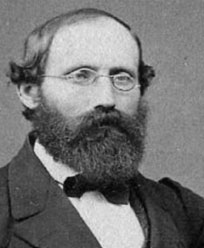
\includegraphics[scale=0.5]{image_chapitres/riemann.jpg}
\unnumberedcaption{Bernhard \textsc{Riemann}} 
\end{wrapfigure}

Malgré ces succès, de nombreuses conjectures restent désespérément
inaccessibles :

\begin{description}[leftmargin=*]
\item[•] La {\em conjecture de \textsc{Goldbach}} : tout nombre pair supérieur à 4 est-il
somme de deux nombres premiers ? On a par exemple : 4=2+2, 6=3+3, 8=5+3, 
10=7+3, 12=7+5, 14=11+3... peut-on toujours décomposer ainsi un nombre pair ?
\item[•] La {\em conjecture des nombres premiers de \textsc{Fermat}} : existe-t-il d'autres
nombres premiers de la forme $F_n=2^{2^n}+1$, à part les 5 que l'on connaît
déjà ($F_0=3$, $F_1=5$, $F_2=17$, $F_3=257$, $F_4=65537$) ? On sait que
pour $n$ entre 5 et 32, $F_n$ n'est pas premier.
\item[•] La {\em conjecture de \textsc{\textbf{Riemann}}} : l'un des problèmes mathématiques actuels
les plus important. Elle concerne les nombres où la fonction zêta de
\textsc{Riemann} s'annule; sa démonstration donnerait la preuve de nombreux
résultats sur la répartition des nombres premiers.  
\item[•] La {\em conjecture des nombres premiers de \textsc{Mersenne}} : existe-t-il une
infinité de nombres premiers de la forme $M_n=2^n-1$ ? On en connaît
49, le dernier, $M_{74~207~281}$, a été trouvé le 7 Janvier 2016, et
c'est le plus grand nombre premier connu à l'heure où l'on écrit
ces lignes (Juin 2016). Vous pouvez participer à la recherche
de ces nombres : 
\PESP{http://www.mersenne.org}


\end{description}




\end{His}

